\section{Results: Controlled Selector Study}

\label{sec:controlled_results}

The controlled study answers RQ4. All six selectors draw from the same frozen
candidate bank under the same token caps and the same whole-item first-fit packing
policy, so differences in this section are attributable to the ordering rule rather
than to representation, acquisition or overflow behaviour. Every interval is a
stratified paired memory-cluster bootstrap over 84 memory episodes with 10{,}000
resamples, and every $p$-value is a paired cluster sign-flip test with Holm
correction across all prespecified comparisons\footnote{The stored statistics use
the documented Holm family across all prespecified full-history and micro accuracy
comparisons. Repeated generations within an episode are averaged before resampling,
so repeated calls do not add independent memory episodes.}.
Negative and inconclusive comparisons are reported alongside the significant ones.

\subsection{The deployed hybrid loses to BM25}

\label{sec:ctrl_main}

Table~\ref{tab:controlled_main} reports accuracy, evidence hit rate and measured
tokens per query for all six selectors at the three budgets. The primary comparison
is hybrid against BM25, and it does not favour the deployed configuration. Hybrid
minus BM25 accuracy is $-36.1$ percentage points at 512 tokens (95\% interval
$[-46.0,-25.8]$; two-sided paired $p=0.0001$, Holm-adjusted $p=0.0021$), $-29.4$
points at 1024 tokens ($[-40.1,-18.3]$; $p=0.0002$, Holm-adjusted $p=0.0022$), and
$-33.7$ points at 2048 tokens ($[-44.0,-23.0]$; $p=0.0001$, Holm-adjusted
$p=0.0021$). The deficit is large, consistent in sign across every budget, and it is
not a marginal result that a different budget or a longer context might quietly
reverse: adding memory does not close the gap, because both selectors receive the
same added budget.

The absolute levels make the size of the reversal concrete. BM25 reaches 68.7\%,
65.9\% and 70.6\% at the three budgets, while the deployed hybrid reaches 32.5\%,
36.5\% and 36.9\%. Two of the controlled variants land where BM25 does. Jaccard
alone reaches 55.2\%, 67.5\% and 71.4\%, and the hybrid with its temporal term
removed reaches 56.7\%, 63.5\% and 70.2\%. Against BM25, the Jaccard-only selector
is statistically indistinguishable at the two larger budgets ($+1.6$ points,
Holm-adjusted $p=1.0000$ at 1024; $+0.8$ points, Holm-adjusted $p=1.0000$ at 2048)
and only modestly behind at 512, where the difference does not survive correction
($-13.5$ points, Holm-adjusted $p=0.1544$). The two weakest selectors are the ones
that ignore query content entirely: prefix ordering reaches 25.0--27.0\% and pure
recency reaches 29.4--32.9\%, both far below BM25 at every budget with Holm-adjusted
$p\le 0.0021$.

Two conclusions follow directly. First, the hybrid's deficit is a property of its
scoring rule, not of the candidate bank or the packing policy, because those are
shared. Second, the near-equality of Jaccard-only and no-time-with-BM25 shows that
lexical ranking over this bank is genuinely competitive; the deployed hybrid is the
outlier, not the lexical family as a whole.

\begin{table}[htbp]
\centering
\small
\caption{Controlled selector study, all selectors and budgets. Accuracy and evidence-hit
columns are percentages over 84 stratified memory episodes; the interval is a stratified
paired memory-cluster bootstrap. Tokens per query excludes offline index construction.
Bold marks the primary comparison.}
\label{tab:controlled_main}
\begin{tabular}{llccc}
\toprule
Selector & Budget & Accuracy (95\% CI) & Evidence hit & Tokens/query \\
\midrule
prefix    & 512  & 27.0 [21.0, 33.3] & 0.0 & 656 \\
recency   & 512  & 29.4 [23.0, 36.1] & 0.0 & 653 \\
jaccard   & 512  & 55.2 [46.8, 63.9] & 66.7 & 686 \\
\textbf{hybrid} & \textbf{512} & \textbf{32.5 [25.4, 40.1]} & \textbf{18.1} & \textbf{663} \\
hybrid\_no\_time & 512 & 56.7 [48.4, 65.5] & 66.7 & 684 \\
bm25      & 512  & 68.7 [60.7, 76.6] & 75.0 & 702 \\
\midrule
prefix    & 1024 & 25.0 [19.8, 30.6] & 0.0 & 1167 \\
recency   & 1024 & 32.9 [25.8, 40.5] & 1.4 & 1169 \\
jaccard   & 1024 & 67.5 [59.1, 75.8] & 77.8 & 1200 \\
\textbf{hybrid} & \textbf{1024} & \textbf{36.5 [29.0, 44.4]} & \textbf{18.1} & \textbf{1182} \\
hybrid\_no\_time & 1024 & 63.5 [55.6, 71.8] & 77.8 & 1198 \\
bm25      & 1024 & 65.9 [58.7, 73.0] & 77.8 & 1224 \\
\midrule
prefix    & 2048 & 25.0 [19.8, 30.6] & 0.0 & 2190 \\
recency   & 2048 & 30.6 [23.8, 38.1] & 0.0 & 2191 \\
jaccard   & 2048 & 71.4 [63.5, 79.4] & 87.5 & 2242 \\
\textbf{hybrid} & \textbf{2048} & \textbf{36.9 [29.4, 45.2]} & \textbf{20.8} & \textbf{2218} \\
hybrid\_no\_time & 2048 & 70.2 [62.3, 78.2] & 87.5 & 2242 \\
bm25      & 2048 & 70.6 [63.1, 78.2] & 84.7 & 2251 \\
\bottomrule
\end{tabular}
\end{table}

\begin{table}[htbp]
\centering
\small
\caption{Paired comparisons from the controlled study. Rows are selector differences in
accuracy points; each interval is a stratified paired memory-cluster bootstrap and each
Holm-adjusted $p$ comes from the corresponding paired cluster sign-flip test. The primary
comparison is hybrid against BM25.}
\label{tab:controlled_pairs}
\begin{tabular}{llccc}
\toprule
Comparison & Budget & Difference (95\% CI) & Holm $p$ & Primary \\
\midrule
hybrid $-$ bm25 & 512  & $-36.1$ $[-46.0,-25.8]$ & $0.0021$ & yes \\
hybrid $-$ bm25 & 1024 & $-29.4$ $[-40.1,-18.3]$ & $0.0022$ & yes \\
hybrid $-$ bm25 & 2048 & $-33.7$ $[-44.0,-23.0]$ & $0.0021$ & yes \\
\midrule
hybrid $-$ hybrid\_no\_time & 512  & $-24.2$ $[-33.7,-14.7]$ & $0.0022$ & no \\
hybrid $-$ hybrid\_no\_time & 1024 & $-27.0$ $[-36.9,-17.5]$ & $0.0021$ & no \\
hybrid $-$ hybrid\_no\_time & 2048 & $-33.3$ $[-42.9,-23.4]$ & $0.0021$ & no \\
\midrule
jaccard $-$ bm25 & 512  & $-13.5$ $[-23.4,-3.2]$  & $0.1544$ & no \\
jaccard $-$ bm25 & 1024 & $+1.6$ $[-6.0,+9.1]$    & $1.0000$ & no \\
jaccard $-$ bm25 & 2048 & $+0.8$ $[-7.1,+8.7]$    & $1.0000$ & no \\
\midrule
prefix $-$ bm25  & 512  & $-41.7$ $[-50.8,-32.1]$ & $0.0021$ & no \\
prefix $-$ bm25  & 1024 & $-40.9$ $[-50.0,-31.7]$ & $0.0021$ & no \\
prefix $-$ bm25  & 2048 & $-45.6$ $[-55.2,-36.1]$ & $0.0021$ & no \\
recency $-$ bm25 & 512  & $-39.3$ $[-50.0,-28.2]$ & $0.0021$ & no \\
recency $-$ bm25 & 1024 & $-32.9$ $[-44.4,-21.4]$ & $0.0021$ & no \\
recency $-$ bm25 & 2048 & $-40.1$ $[-50.4,-29.4]$ & $0.0021$ & no \\
\bottomrule
\end{tabular}
\end{table}

\FloatBarrier

\subsection{Evidence delivery orders the same way as accuracy}

\label{sec:ctrl_evidence}

Accuracy is a downstream measure that depends on the answering model as well as on
retrieval, so it is worth asking whether the retrieval step itself displays the same
ordering. It does. The evidence-hit column of Table~\ref{tab:controlled_main} tracks
the accuracy column closely: BM25 delivers complete annotated evidence for 75.0\%,
77.8\% and 84.7\% of episodes, Jaccard and no-time for 66.7--87.5\%, and the deployed
hybrid for only 18.1\%, 18.1\% and 20.8\%. Prefix and recency deliver essentially no
complete evidence at any budget (0.0--1.4\%).

The full-history sweep over all 500 LongMemEval-S histories, which calls no language
model, sharpens the picture because it removes the answering model from the loop.
Across 9000 selector/budget traces and 470 eligible non-abstention histories,
evidence-session recall is 80.4\%, 86.2\% and 91.8\% for BM25 at the three budgets,
69.7--89.5\% for Jaccard and no-time, and 24.4\%, 28.5\% and 32.2\% for the deployed
hybrid. Complete annotated-turn coverage, the strictest of the reported retrieval
metrics, is 46.6\% for BM25 at 512 tokens against 12.1\% for the hybrid. Every
retrieval metric in the sweep agrees with the accuracy ordering from the controlled
question set, which is what one would expect if the deficit originates in candidate
ordering rather than in the generation or grading stages.

\begin{table}[htbp]
\centering
\small
\caption{Full-history retrieval sweep over 500 LongMemEval-S histories with no language
model in the loop; 470 non-abstention histories enter the denominators. Values are
percentages. These are retrieval metrics, not answer accuracy, and they do not establish
semantic delivery of every answer fact.}
\label{tab:full500}
\begin{tabular}{lcccccc}
\toprule
Budget & Selector & Session & Turn & Char. & Complete \\
       &          & recall  & recall & cov. & turns \\
\midrule
512  & bm25           & 80.4 & 63.0 & 61.7 & 46.6 \\
512  & jaccard        & 69.7 & 46.1 & 44.5 & 34.3 \\
512  & hybrid\_no\_time & 69.7 & 46.1 & 44.5 & 34.3 \\
512  & hybrid         & 24.4 & 17.9 & 17.6 & 12.1 \\
512  & recency        & 4.0  & 1.9  & 1.7  & 0.9 \\
512  & prefix         & 2.0  & 0.6  & 0.7  & 0.2 \\
\midrule
1024 & bm25           & 86.2 & 72.0 & 71.4 & 59.1 \\
1024 & jaccard        & 79.9 & 57.5 & 55.8 & 45.7 \\
1024 & hybrid\_no\_time & 79.9 & 57.5 & 55.8 & 45.7 \\
1024 & hybrid         & 28.5 & 22.5 & 22.1 & 16.6 \\
1024 & recency        & 4.2  & 2.2  & 2.1  & 1.1 \\
1024 & prefix         & 2.3  & 1.0  & 1.1  & 0.2 \\
\midrule
2048 & bm25           & 91.8 & 78.4 & 77.8 & 67.2 \\
2048 & jaccard        & 89.5 & 68.8 & 67.6 & 57.7 \\
2048 & hybrid\_no\_time & 89.5 & 68.8 & 67.6 & 57.7 \\
2048 & hybrid         & 32.2 & 26.3 & 25.9 & 20.4 \\
2048 & recency        & 4.9  & 3.5  & 3.4  & 2.1 \\
2048 & prefix         & 2.3  & 1.6  & 1.6  & 0.2 \\
\bottomrule
\end{tabular}
\end{table}

\begin{figure}[htbp]\centering
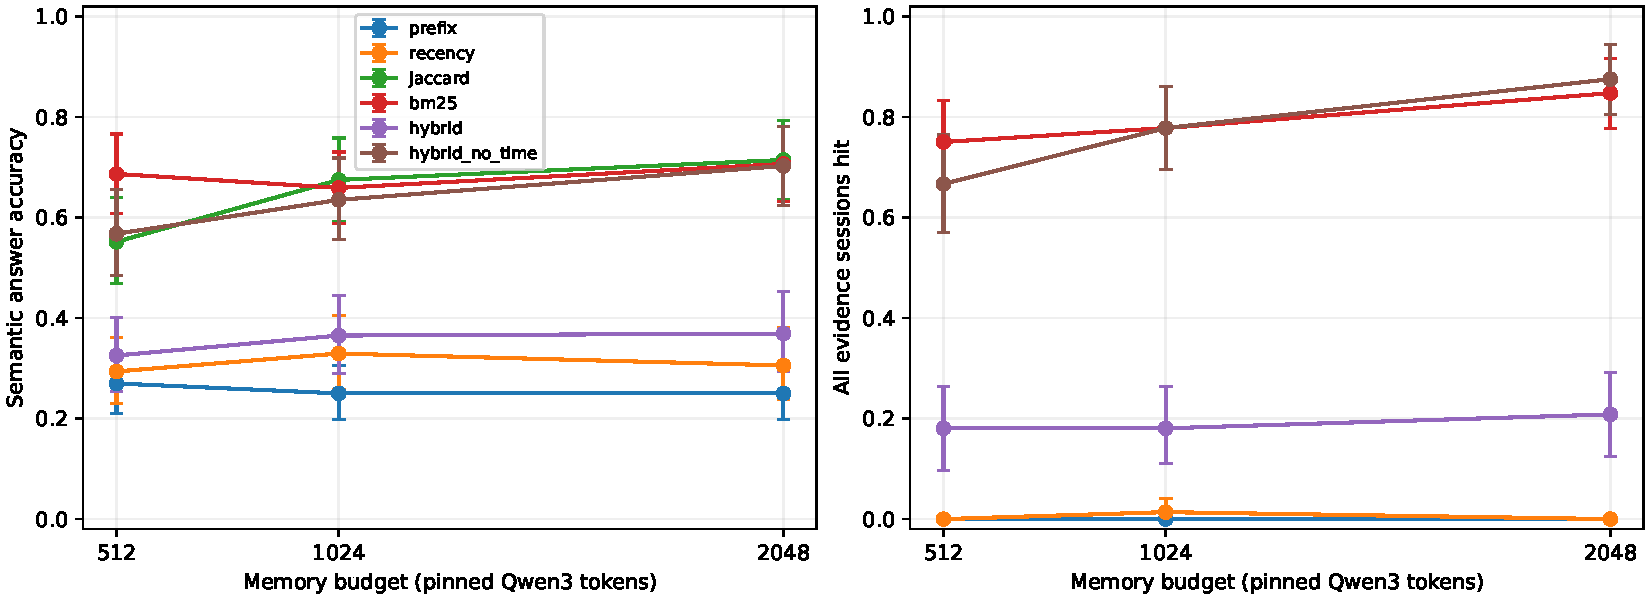
\includegraphics[width=\linewidth]{figures/fair_baselines.pdf}
\caption{Controlled comparison across memory budgets. The left panel reports semantic
answer accuracy and the right panel reports the fraction of episodes whose evidence
sessions are delivered, for all six selectors. Intervals are stratified paired
memory-cluster bootstraps over the same 84 episodes at each budget. Sharing the
candidate bank and packing policy across arms makes the separation between the
deployed hybrid and the lexical selectors attributable to ordering.}
\label{fig:fair}\end{figure}

\begin{figure}[htbp]\centering
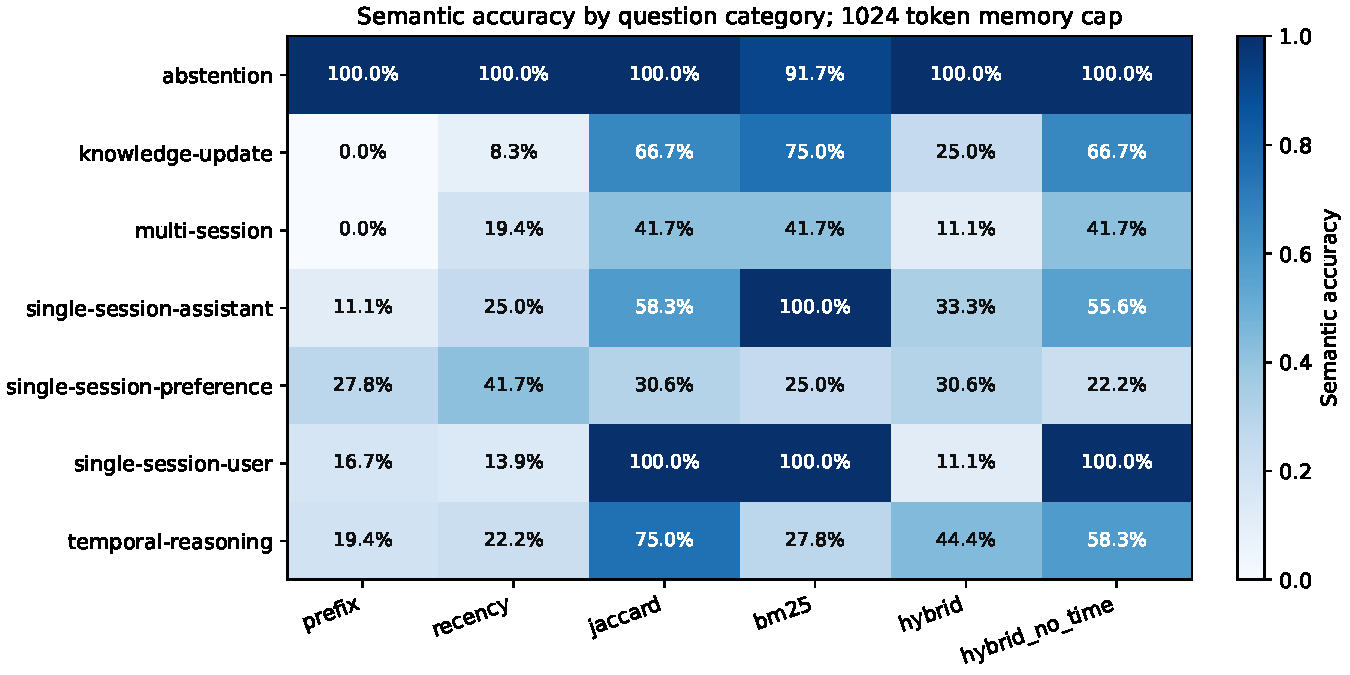
\includegraphics[width=\linewidth]{figures/category_accuracy.pdf}
\caption{Semantic accuracy by question category at the 1024-token budget. Categories are
the LongMemEval-S strata; each cell holds twelve questions. The deployed hybrid's deficit
is broad rather than confined to a single category, and it is most severe in
single-session factual recall, where BM25 answers 100\% of the questions and the hybrid
answers 11.1\%.}
\label{fig:category}\end{figure}

\FloatBarrier

\subsection{Category-level behaviour}

\label{sec:ctrl_category}

Table~\ref{tab:categories} reports per-category accuracy at the 1024-token budget. The
deployed hybrid's deficit is not confined to one stratum. It is most severe exactly
where memory retrieval should be easiest to get right: on single-session-user
questions, which ask for a fact stated directly in one session, BM25 answers 100.0\%
of the twelve questions while the deployed hybrid answers 11.1\%. On
single-session-assistant questions the gap runs the same way (100.0\% against
33.3\%). The hybrid's only consistent advantage by category is abstention, where it
reaches 100.0\% against BM25's 91.7--91.7\% range; both selectors are near ceiling on
that stratum, so the difference is small in absolute terms.

Two strata are difficult for every selector. Multi-session questions, which require
combining facts across several sessions, peak at 50.0\% and are answered at 41.7\%
by BM25 and 11.1\% by the hybrid at 1024 tokens. Temporal-reasoning questions peak at
75.0\% for Jaccard. Both strata plausibly stress the frozen single-layer bank more
than they stress the ordering rule, since neither the bank nor the packing policy
allows cross-session consolidation, and we do not read the category table as
evidence about selector behaviour on those strata beyond what the confidence
intervals support. Each cell holds twelve questions, so category-level differences
carry wide intervals and we treat the table as descriptive.

\begin{table}[htbp]
\centering
\small
\caption{Semantic accuracy by question category at the 1024-token budget. Each cell is a
percentage over twelve questions in that stratum. Cells are descriptive; with twelve
questions per stratum the intervals are wide, and the table is not used for significance
claims.}
\label{tab:categories}
\begin{tabular}{lcccccc}
\toprule
Category & prefix & recency & jaccard & hybrid & hybrid\_no\_time & bm25 \\
\midrule
single-session-user        & 16.7 & 13.9 & 100.0 & 11.1 & 100.0 & 100.0 \\
single-session-assistant   & 11.1 & 25.0 & 58.3  & 33.3 & 55.6  & 100.0 \\
single-session-preference  & 27.8 & 41.7 & 30.6  & 30.6 & 22.2  & 25.0 \\
knowledge-update           & 0.0  & 8.3  & 66.7  & 25.0 & 66.7  & 75.0 \\
temporal-reasoning         & 19.4 & 22.2 & 75.0  & 44.4 & 58.3  & 27.8 \\
multi-session              & 0.0  & 19.4 & 41.7  & 11.1 & 41.7  & 41.7 \\
abstention                 & 100.0 & 100.0 & 100.0 & 100.0 & 100.0 & 91.7 \\
\bottomrule
\end{tabular}
\end{table}

\FloatBarrier

\subsection{Component controls and measured reuse}

\label{sec:ctrl_controls}

Two mechanism controls use an adapted twenty-item workload in which the required
fact-item recall, rather than the full-history bank, defines success. Both compare a
variant against hybrid on raw exchanges and are mechanism controls over twenty
adapted episodes; they do not establish full-history generality.

Replacing raw exchanges with model-acknowledged exchanges has no measurable effect.
The adapted control hybrid\_model\_ack minus hybrid\_raw has an accuracy difference
of $+0.0$ points at 1024 tokens (95\% interval $[+0.0,+0.0]$; Holm-adjusted
$p=1.0000$) and $+0.0$ at 2048 tokens. The representation-difference control
hybrid\_exchange minus hybrid\_raw is $-36.7$ points at 512 tokens (Holm-adjusted
$p=0.0324$), $-16.7$ points at 1024 tokens (Holm-adjusted $p=0.8728$) and $+0.0$ at
2048 tokens. That control changes exchange formatting, which affects both lexical
features and token packing at once, so it does not isolate packing from lexical
content; we report it as a joint representation control. At the two larger budgets
all three variants reach 100.0\% on the adapted workload, which is consistent with the
workload being easier than the full-history bank and with the adapted controls
lacking the power to detect differences at those budgets.

The write-cost question is separate from the ranking question, but the same
experiment set measures it. Because the reuse suite builds one memory bank and then
serves one, five, ten and twenty distinct queries from it, it amortises construction
rather than extrapolating from a single query. Measured write-plus-query tokens per
query are 500.9, 499.4, 498.8 and 498.8 for bm25\_raw; 2569.5, 913.1, 705.7 and 602.3
for hybrid\_model\_ack; and 501.0, 499.4, 498.9 and 498.8 for hybrid\_raw. All three
arms reach 100.0\% accuracy on the synthetic reuse banks. The pattern is the useful
part: the file-style and raw-hybrid arms are essentially flat in the number of
queries served, while the model-acknowledged arm starts more than five times more
expensive and converges towards the others only after twenty queries share one
build. Construction cost is therefore amortisable, and the synthetic banks share
templates, so the absolute levels should not be read as general natural-workload
costs.

\begin{figure}[htbp]\centering
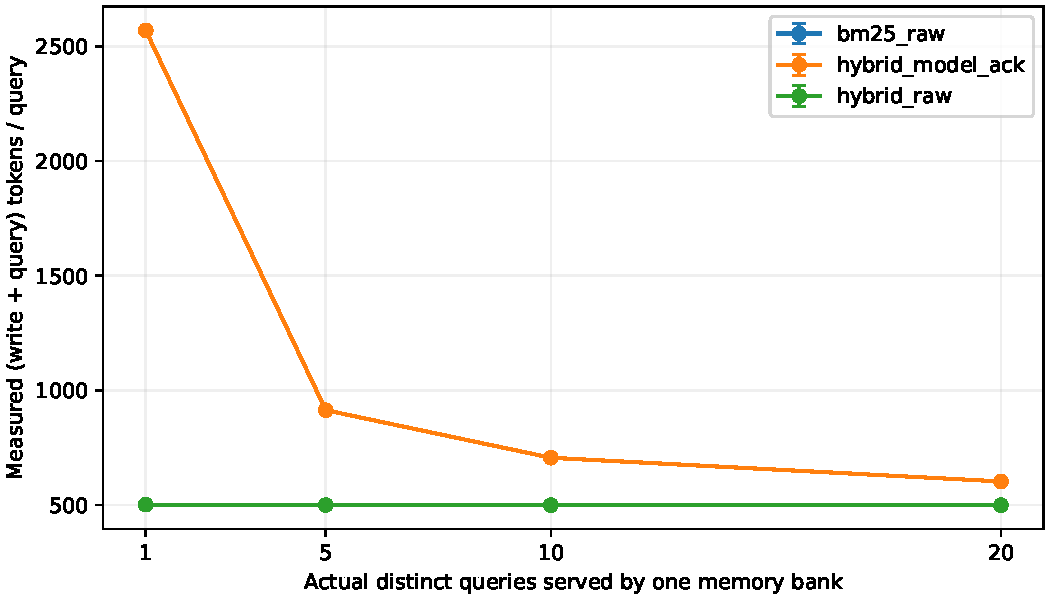
\includegraphics[width=0.8\linewidth]{figures/memory_reuse.pdf}
\caption{Measured write-plus-query tokens per query as one memory bank serves one, five,
ten and twenty distinct queries. The model-acknowledged arm amortises construction cost
across queries and converges towards the direct-write arms; the direct-write arms are
essentially flat. All arms reach 100\% accuracy on these synthetic banks, so this figure
concerns cost rather than quality.}
\label{fig:reuse}\end{figure}

\FloatBarrier

\subsection{Grading robustness}

\label{sec:ctrl_grading}

Because accuracy in this study is produced by a substituted judge, a natural objection
is that the deficit is an artefact of grading. The audit limits how much can be claimed
in either direction, so we state it precisely. Of the audited generations, 239 were
flagged as primary/secondary judge disagreements across the 966-review queue, and
those have received boolean human decisions. Replacing only the reviewed labels while
holding all unreviewed primary labels fixed moves the 512-token figures from 68.7\% to
62.3\% for BM25 and from 32.5\% to 22.6\% for the hybrid. Under that substitution the
hybrid remains far behind BM25 at 512 tokens, and the bounds that vary only the known
disagreements (61.9--69.0\% for BM25 against 22.6--32.5\% for the hybrid) do not
overlap. The direction of the controlled result therefore does not depend on the
reviewed subset of label decisions.

This is a bounded statement, not a validation of the judge. The substitution holds all
unaudited labels fixed and varies only known disagreements, so it is descriptive rather
than a full second-judge evaluation or a bound on all grading errors. Roughly
three-quarters of the review queue remains unaudited, and we do not claim the primary
judge agrees with human judgement on that remainder. It is also worth noting that a
grading artefact would have to be selector-specific to produce the observed pattern,
since all six selectors were graded by the same pinned prompts and the same parser;
a general grading bias would move the selectors together rather than separating the
hybrid from BM25.

\begin{figure}[htbp]
\centering
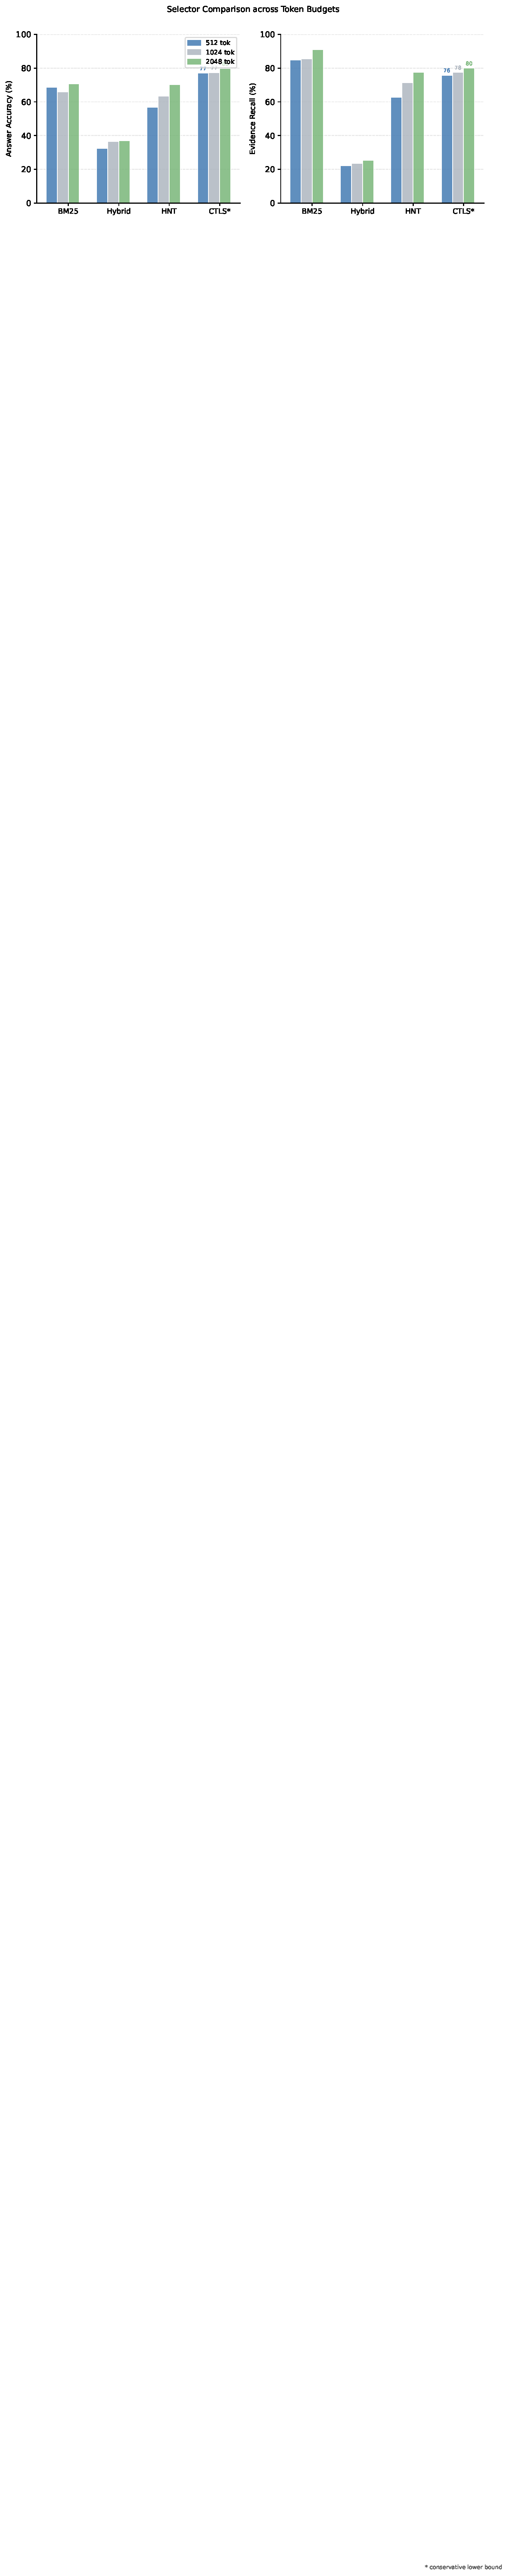
\includegraphics[width=\linewidth]{figures/selector_comparison.pdf}
\caption{All six selectors across three token budgets on the stratified LongMemEval-S subset.
The primary comparison (BM25 vs.\ deployed hybrid) is highlighted with raw percentage-point
gap annotations. Prefix and recency, which ignore query content, are the weakest selectors.
Jaccard-only and hybrid\_no\_time land near BM25 at the larger budgets, confirming that
the temporal term -- not the lexical component -- drives the hybrid deficit.}
\label{fig:selector_comparison}
\end{figure}

\begin{figure}[htbp]
\centering
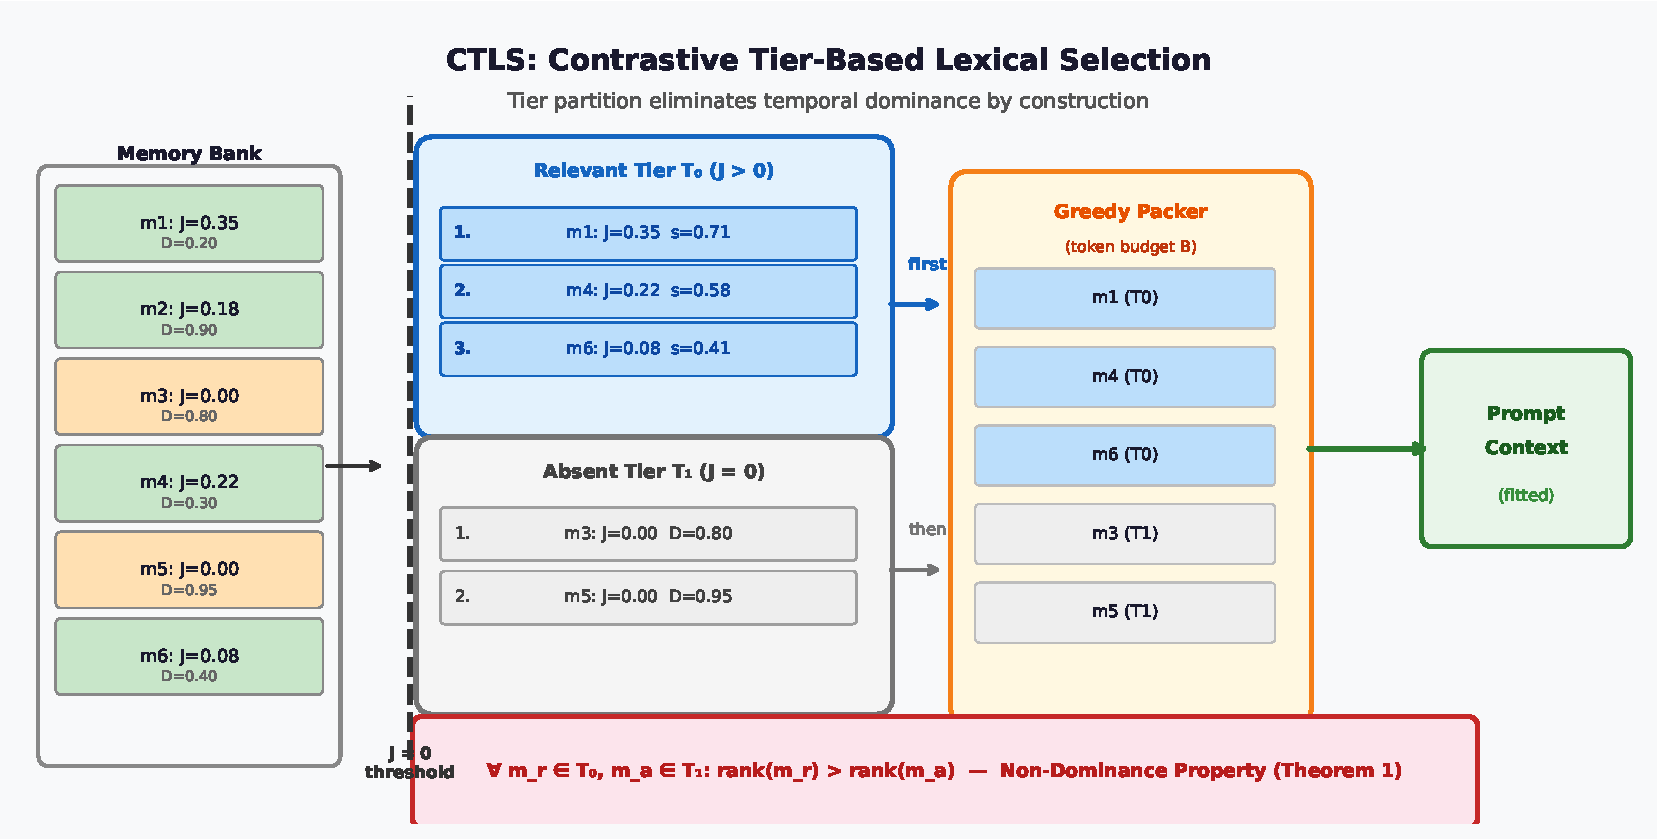
\includegraphics[width=\linewidth]{figures/ctls_concept.pdf}
\caption{CTLS tier partition. The memory bank is divided at the J=0 threshold before scoring.
Relevant-tier items (positive Jaccard overlap, blue) are ranked by full hybrid score and
packed first. Absent-tier items (zero overlap, gray) are packed afterward. The
Non-Dominance Property (bottom box) guarantees that no absent-tier item can displace a
relevant-tier item regardless of temporal decay values or weight settings.}
\label{fig:ctls_concept}
\end{figure}

\FloatBarrier
